\subsection{LQ Controllers}
\label{subsec:lq_controllers}
Linear Quadratic (LQ) Controllers are optimal controllers that use state-space representation. These kinds of models minimize a quadratic cost function that balances state performance and control effort, providing a systematic way to design efficient and stable controllers.

Hereafter the Linear Quadratic Regulator (LQR), its expansion with tracking and Linear Quadratic Integrator (LQI) are taken into account to develop a stable controller for our system.

\subsubsection{LQR}
\label{subsubsec:lqr}
The Linear Quadratic Regulator (LQR) is a full state feedback controller. In order to provide the optimal control to the system, the controller aims to minimize the cost function $\mathcal{J}$ (Equation \ref{cost function}). The feedback control gain matrix $\mathbf{K}$ is thus computed considering the closed-loop characteristics that are relevant to us, specifically how efficient must be the and how much effort can be spent to get the desired performance.

The cost function which we aim to minimize is $\mathcal{J}$:

\begin{equation}
    \mathcal{J} = \int_0^\infty \mathbf{x}(t)^\top \mathbf{Q} \mathbf{x}(t) + \mathbf{u}(t)^\top \mathbf{R} \mathbf{u}(t) dt,
    \label{cost function}
\end{equation}

where $\mathbf{Q}$ is a positive semi-definite matrix penalizing state deviations from the desired state, and $\mathbf{R}$ is a positive semi-definite matrix penalizing control effort.

The optimal control input is given by:
\begin{equation}
    \mathbf{u}(t) = -\mathbf{K} \mathbf{x}(t),
\end{equation}

where the feedback gain $\mathbf{K}$ is determined by solving the Algebraic Riccati Equation:
\begin{equation}
    \mathbf{A}^\top \mathbf{P} + \mathbf{P}\mathbf{A} - \mathbf{P}\mathbf{B}\mathbf{R}^{-1} \mathbf{B}^\top \mathbf{P} + \mathbf{Q} = 0,
\end{equation}

where $\mathbf{P}$ is the positive semi-definite solution to the ARE.

Once $\mathbf{P}$ is computed, the feedback gain matrix $K$ is:
\begin{equation}
    \mathbf{K} = \mathbf{R}^{-1} \mathbf{B}^\top \mathbf{P}.
\end{equation}

The closed-loop system dynamics under the LQR controller are:
\begin{equation}
    \mathbf{\dot{x}}(t) = \mathbf{(A - B K)}\mathbf{x}(t).
\end{equation}

\paragraph{Design} In order to develop an efficient controller, a great attention has been posed on the estimation of the matrices $\mathbf{Q}$ and $\mathbf{R}$. As far as concerned the $\mathbf{Q}$ matrix, the main relevance was attributed on the values that influence the state position and a moderate relevance on the values that influence the control input. Moreover, some values for $R$ have been estimated considering inherent literature parameters.

\begin{equation}
    \mathbf{Q} =
    \begin{bmatrix}
        25e^3 & 0 & 0 \\ 0 & 0 & 0\\ 0 & 0 & 16e^{-2}
    \end{bmatrix}
    \quad
    \mathbf{R} = 0.5
\end{equation}

Under these assumptions the following gain matrix has been computed.
\begin{equation}
    \mathbf{K} =
    \begin{bmatrix}
        -371.72 & -7.53 & 1.53
    \end{bmatrix}
\end{equation}

The poles of the system have been computed in order to analyze its stability:

\begin{equation}
    eig\mathbf{(A-BK)} =
    \begin{bmatrix}
        -47.51 + 52.95i \\
        -47.51 - 52.95i \\
        -92.90 + 0i
    \end{bmatrix}
\end{equation}

Since eigenvalues of matrix $\mathbf{(A-BK)}$ are situated in left hand-side plan, the resulting system is stable. Neverthless, this control strategy has some limitations that restrict its effectiveness. Indeed, LQR does not inherently provide steady-state error correction for systems with constant disturbances or setpoint changes. It was thus impossible to make the system follows a reference input as in the other examples. In order to do that, some extensions of this simpler controller have been developed and reported in the next sections.

\subsubsection{LQR with tracking capabilities}
\label{subsubsec:lqr_tracking}

The Linear Quadratic Regulator (LQR) with tracking capabilities extends the classical LQR framework to manage systems where the goal is not only to stabilize the system but also to ensure it follows a desired trajectory or reaches a specified setpoint. This advanced control strategy is particularly useful in applications involving reference tracking, where the control objective dynamically changes over time.

To account for tracking, the state-space representation is augmented to include the tracking error:

\begin{equation}
    \mathbf{z} = \begin{bmatrix} \mathbf{x} \\ \mathbf{e} \end{bmatrix},
\end{equation}

where $\mathbf{x}$ is the system state vector, and $\mathbf{e}$ is the error between the system state and the desired reference trajectory.

The cost function for the LQR with tracking is defined as:

\begin{equation}
    \mathcal{J} = \int_0^\infty (\mathbf{z}^\top \mathbf{Q_z} \mathbf{z} + \mathbf{u}^\top \mathbf{R} \mathbf{u} ) dt,
\end{equation}

where $\mathbf{Q_z}$ is the positive semi-definite weighting matrix for the augmented state, and $\mathbf{R}$ is a positive definite weighting matrix for the control input.

The augmented system dynamics are given by:

\begin{equation}
    \mathbf{\dot{z}} = \mathbf{A_z} \mathbf{z} + \mathbf{B_z} \mathbf{u},
\end{equation}

where $\mathbf{A_z}$ and $\mathbf{B_z}$ are derived from the original state-space model:

\begin{equation}
    \mathbf{A_z} = \begin{bmatrix} A & 0 \\ -A_{\text{ref}} & 0 \end{bmatrix}, \quad
    \mathbf{B_z} = \begin{bmatrix} B \\ 0 \end{bmatrix}.
\end{equation}

The optimal control law is derived as:

\begin{equation}
    \mathbf{u}(t) = -\mathbf{K} \mathbf{z}(t),
\end{equation}

where $\mathbf{K}$ is the feedback gain matrix, computed by solving the Riccati equation for the augmented system:

\begin{equation}
    \mathbf{P_z} \mathbf{A_z} + \mathbf{A_z}^\top \mathbf{P_z} - \mathbf{P_z} \mathbf{B_z} \mathbf{R}^{-1} \mathbf{B_z}^\top \mathbf{P_z} + \mathbf{Q_z} = 0.
\end{equation}

This approach ensures accurate reference tracking, balances control effort and tracking performance through the tuning of $\mathbf{Q_z}$ and $\mathbf{R}$, and is robust to disturbances and modeling inaccuracies.

\paragraph{Design} The LQR with reference tracking has been developed using the same matrices $\mathbf{Q}$ and $\mathbf{R}$ described in Subsection \ref{subsubsec:lqr}, with the addiction of the part related to the tracking error.

\paragraph{Step Response} The experimental data measured from system controlled by LQR tracking are reported below. The reference state is followed observing a small gap after the application of the step signal.

\begin{figure}[H]
    \centering
    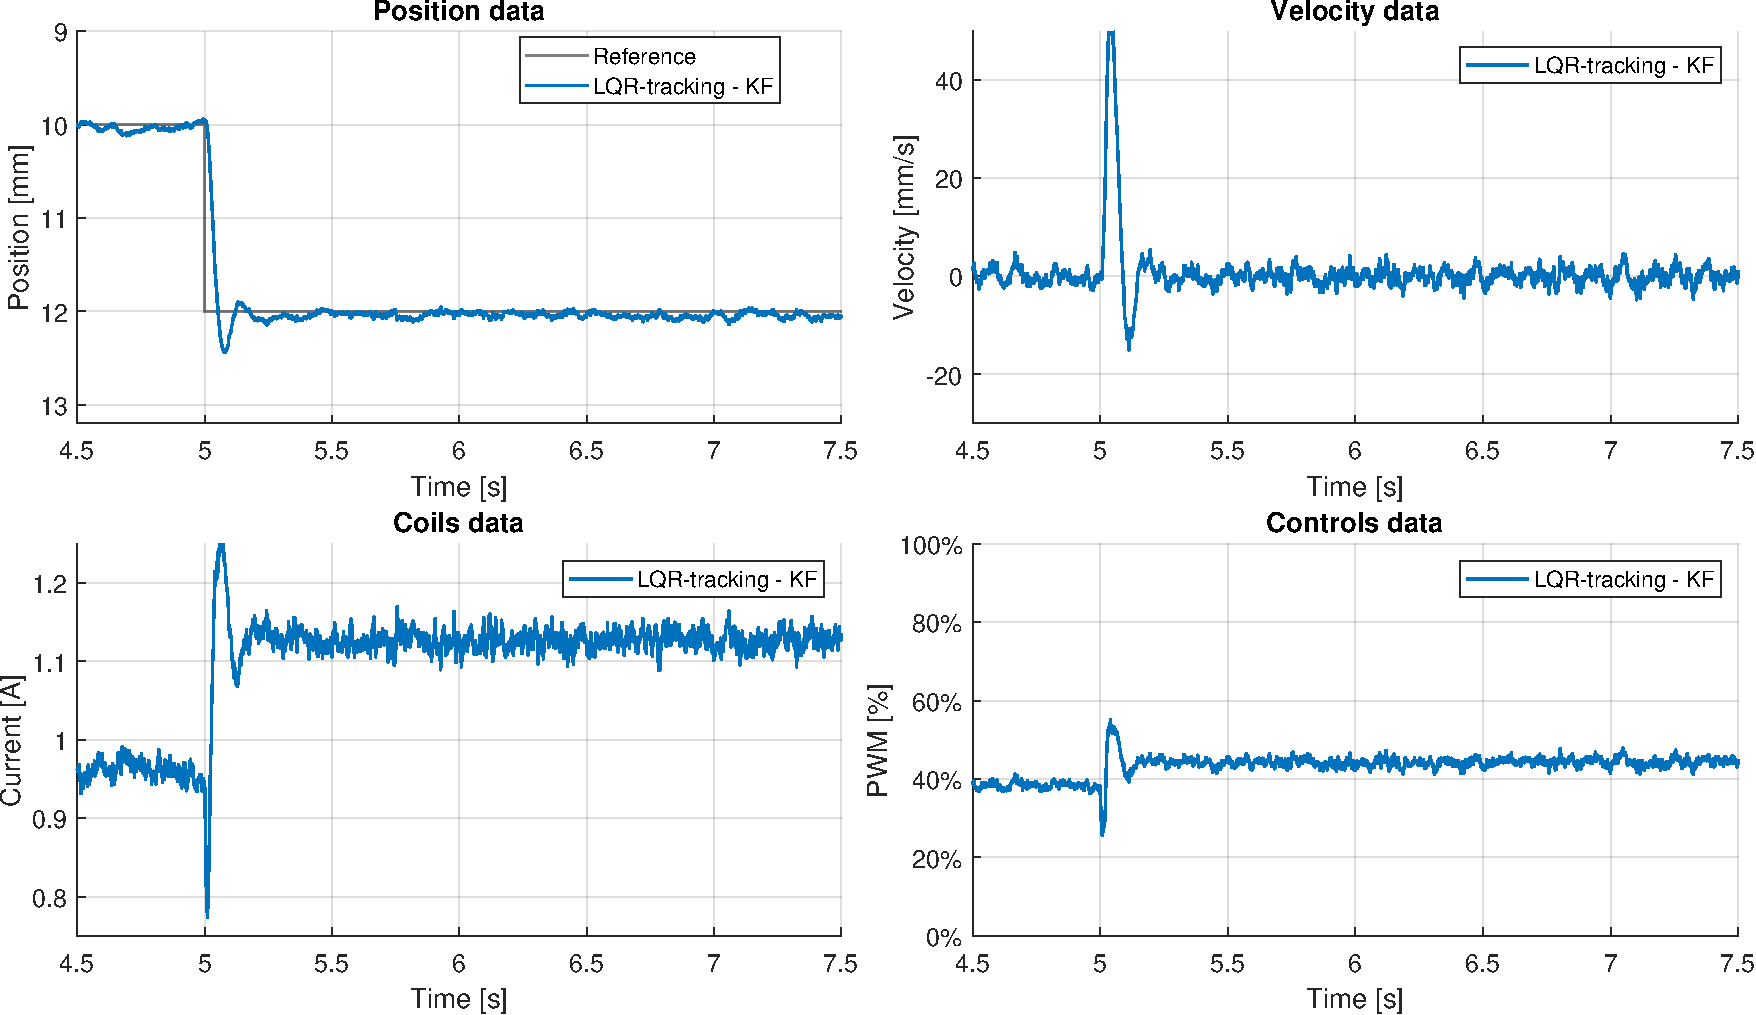
\includegraphics[width=1\linewidth]{./img/MATLAB/results/step_LQR_tracking_KF.pdf}
    \caption{Step Response}
    \label{fig:Step Response}
\end{figure}

\subsubsection{LQI}
\label{subsubsec:lqi}
The Linear Quadratic Integrator (LQI) is an extension of the classical LQR to achieve reference tracking and disturbance rejection by augmenting the system with integral states. Below are the key equations involved.

The augmented state-space model includes the integral of the output error:

\begin{equation}
    \begin{aligned}
        \mathbf{\dot{x}}(t) = \mathbf{A} \mathbf{x}(t) + \mathbf{B} \mathbf{u}(t), \\ \mathbf{\dot{z}}(t) = \mathbf{C} \mathbf{x}(t) - \mathbf{r}(t),
    \end{aligned}
\end{equation}

where $\mathbf{x}(t)$ is the state vector, $\mathbf{u}(t)$ is the control input, $\mathbf{r}(t)$ is the reference signal, and $\mathbf{z}(t)$ is the integral of the tracking error.

The augmented system can be written as:
\begin{equation}
    \begin{bmatrix}
        \mathbf{\dot{x}}(t) \\
        \mathbf{\dot{z}}(t)
    \end{bmatrix}
    =
    \begin{bmatrix}
        \mathbf{A} & 0 \\
        \mathbf{C} & 0
    \end{bmatrix}
    \begin{bmatrix}
        \mathbf{x}(t) \\
        \mathbf{z}(t)
    \end{bmatrix}
    +
    \begin{bmatrix}
        \mathbf{B} \\
        0
    \end{bmatrix}
    \mathbf{u}(t).
\end{equation}

The cost function to be minimized is:
\begin{equation}
    J = \int_0^\infty \left(
    \begin{bmatrix}
            \mathbf{x}(t) \\
            \mathbf{z}(t)
        \end{bmatrix}^\top
    \begin{bmatrix}
            \mathbf{Q_x} & 0            \\
            0            & \mathbf{Q_z}
        \end{bmatrix}
    \begin{bmatrix}
            \mathbf{x}(t) \\
            \mathbf{z}(t)
        \end{bmatrix}
    + \mathbf{u}(t)^\top \mathbf{R} \mathbf{u}(t)
    \right) dt,
\end{equation}
where $\mathbf{Q_x}$ is the state weighting matrix, $\mathbf{Q_z}$ is the integral state weighting matrix, and $\mathbf{R}$ is the control effort weighting matrix. The optimal control input is:

\begin{equation}
    \mathbf{u}(t) = -\mathbf{K}
    \begin{bmatrix}
        \mathbf{x}(t) \\
        \mathbf{z}(t)
    \end{bmatrix},
\end{equation}

where $\mathbf{K}$ is the feedback gain matrix obtained from solving the Algebraic Riccati Equation (ARE) for the augmented system.

The feedback gain $\mathbf{K}$ is partitioned as:
\begin{equation}
    \mathbf{K} =
    \begin{bmatrix}
        \mathbf{K_x} & \mathbf{K_z}
    \end{bmatrix},
\end{equation}
where $\mathbf{K_x}$ corresponds to the state feedback, and $\mathbf{K_z}$ corresponds to the integral action.

\paragraph{Design} As for the LQR, the $\mathbf{Q}$ and the $\mathbf{R}$ matrices have been estimated in order to implement the LQI controller. The weighting parameters are the same except for the additional contribution which characterizes a huge relevance on the tracking error.

\begin{equation}
    \begin{aligned}
        \mathbf{Q} & =
        \begin{bmatrix}
            25e^3 & 0 & 0        & 0      \\
            0     & 0 & 0        & 0      \\
            0     & 0 & 16e^{-2} & 0      \\
            0     & 0 & 0        & 10^{6}
        \end{bmatrix},  \quad
        \mathbf{R} & = 0.5.
    \end{aligned}
\end{equation}

The feedback gain matrix  $\mathbf{K}$ is thus been computed:

\begin{equation}
    \begin{aligned}
        \mathbf{K} & =
        \begin{bmatrix}
            -513.31 & -9.19 & 1.71 & 4472.13
        \end{bmatrix}.
    \end{aligned}
\end{equation}

Finally, the following eigenvalues have been computed to ensure control stability:

\begin{equation}
    \begin{aligned}
        eig\mathbf{(A-BK)}  =
        \begin{bmatrix}
            -19.74 + 0i     \\
            -46.54 + 53.49i \\
            -46.54 - 53.49i \\
            -92.40 + 0i
        \end{bmatrix}.
    \end{aligned}
\end{equation}

\paragraph{Step Response} The measured data are reported in Figure \ref{fig:Step Response} to exhibit the behavior of the system state correspondent to the application of a step signal.

\begin{figure}[H]
    \centering
    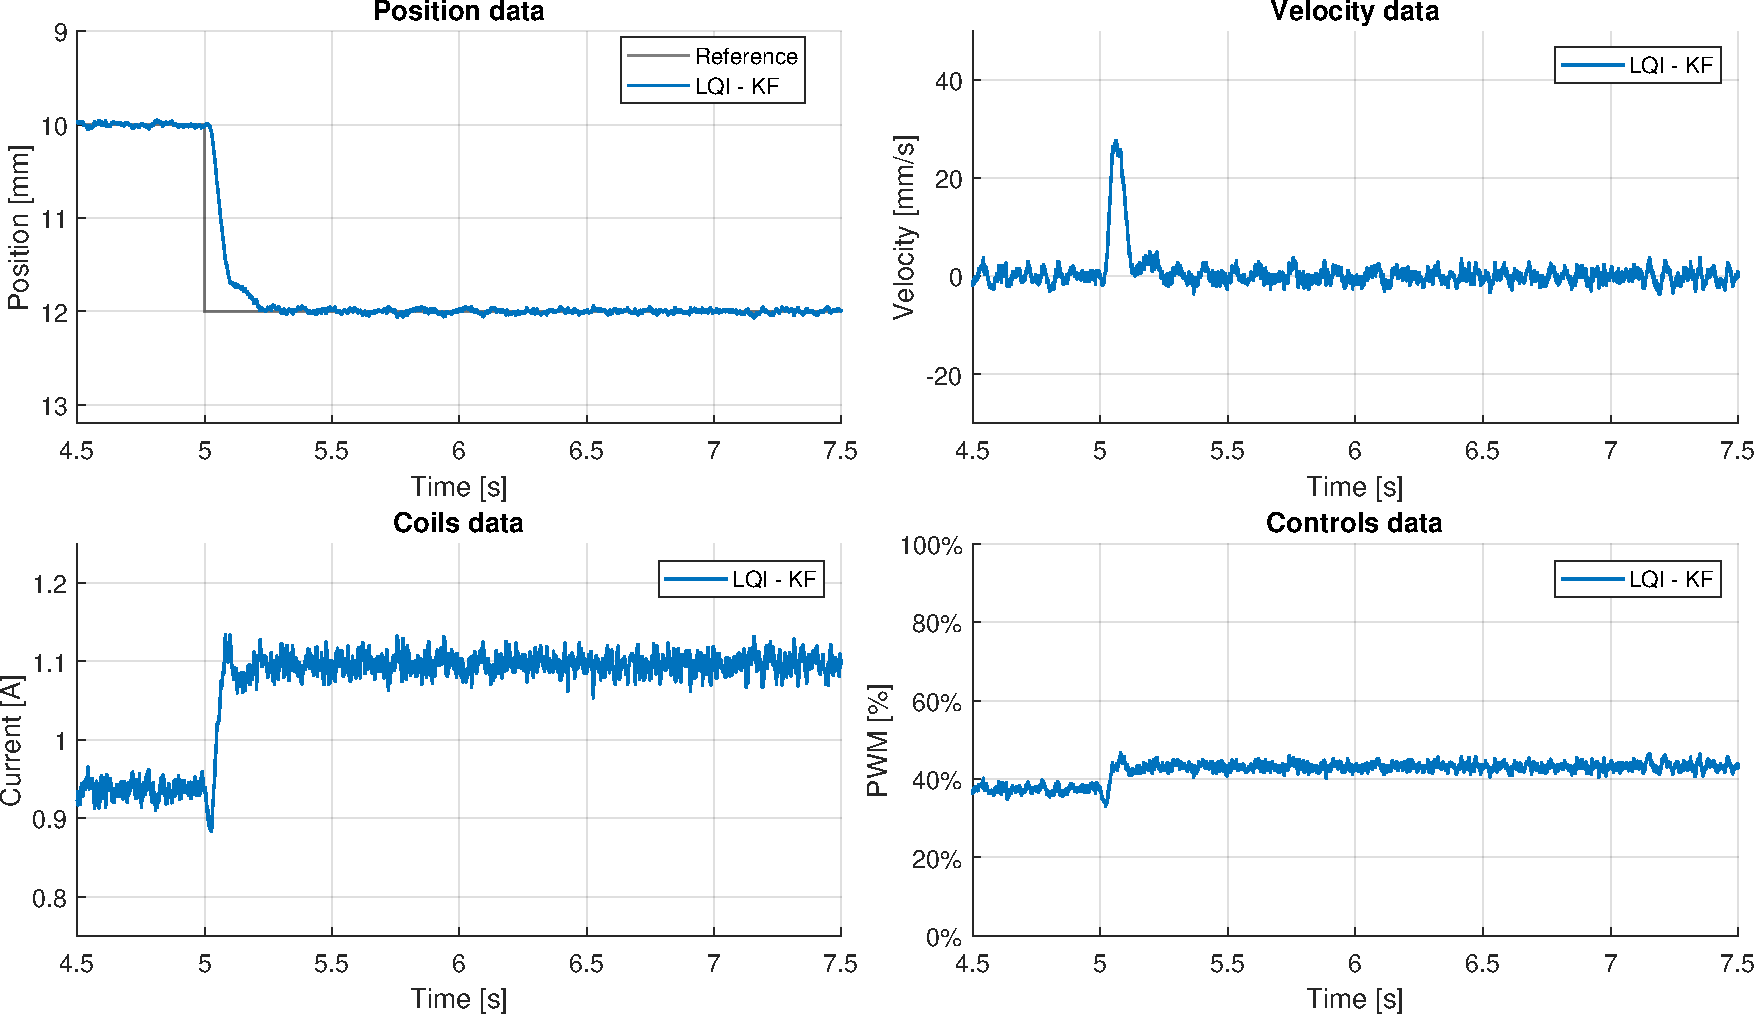
\includegraphics[width=1\linewidth]{./img/MATLAB/results/step_LQI_KF.pdf}
    \caption{Step Response}
    \label{fig:Step Response}
\end{figure}
